%%%%%%%%%%%%%% COPYRIGHT INFORMATION %%%%%%%%%%%%%%
% Template by
% Author: Sascha Frank 
% Nov. 2006
% University Freiburg 
% www.informatik.uni-freiburg.de/~frank/
% Distributed freely for non-commercial use

%%%%%%%%%%%%%%%%%%%%% PREAMBLE %%%%%%%%%%%%%%%%%%%%%
\documentclass{beamer}
\usepackage{beamerthemeshadow}
\usepackage{lmodern}
\usepackage{color}
\usepackage[]{url}

% include frame number on each frame
\setbeamertemplate{footline}{\quad \insertframenumber/\inserttotalframenumber}
\newcommand{\cmark}{\ding{51}} % check-mark
\newcommand{\xmark}{\ding{55}} % X-mark
\newcommand{\inv}{^{-1}}
\newcommand{\e}{\varepsilon}
\newcommand{\E}{\mathbb{E}}
\newcommand{\N}{\mathbb{N}}
\newcommand{\C}{\mathcal{C}}
\newcommand{\M}{\mathcal{M}}
\renewcommand{\P}{\mathbb{P}}
\newcommand{\R}{\mathbb{R}}
\newcommand{\Var}{\mathbb{V}}
\newcommand{\X}{\mathcal{X}}
\newcommand{\Y}{\mathcal{Y}}
\newcommand{\Z}{\mathcal{Z}}
\newcommand{\dist}{\operatorname{dist}}
\newcommand{\vi}{{\vec i}}
\newcommand{\sminus}{\backslash}

%%%%%%%%%%%%%%%%%%%%% DOCUMENT %%%%%%%%%%%%%%%%%%%%%
\begin{document}
\title{Constraints and Metric Learning\\in Semi-Supervised Clustering}
\author[Singh]{Shashank Singh
\footnote{Carnegie Mellon University, Pittsburgh, PA, USA}
}
\institute{11-745 New Methods in Large-Scale Structured Learning}
\date{October 21, 2014}

\section{Introduction}
\frame{\titlepage}

\subsection{Motivations}

\frame{\frametitle{Two Papers}
\begin{columns}[T] % align columns
\begin{column}{.52\textwidth}
Xing et al., 2002,
Distance Metric Learning, with application to Clustering with side-information
\begin{itemize}
\item first learn metric from labeled data (``preprocessing step''), and then
cluster
\item single metric for all data
\item obey all constraints
\end{itemize}
\end{column}%
\hfill%
\begin{column}{.52\textwidth}
Bilenko et al., 2004,
Integrating Constraints and Metric Learning in Semi-Supervised Clustering
\begin{itemize}
\item leverage unlabeled data for metric learning by alternating clustering and
metric learning
\item separate metric for each cluster
\item soft constraints tolerate noisy supervision
\end{itemize}
\end{column}
\end{columns}
}

\subsection{Constraints}
\frame{\frametitle{Constraints}
Allow constraints of the form:
\[\ell_i = \ell_j
    \quad \mbox{ and } \quad
    \ell_i \neq \ell_j,
\]
where $\ell_i$ denotes the label of $x_i$.
\vspace{5mm}

Define ``must-link'' and ``cannot-link'' sets
\[\M := \{(i,j) : \ell_i = \ell_j \mbox{ is a constraint}\}\]
and
\[\C := \{(i,j) : \ell_i \neq \ell_j \mbox{ is a constraint}\}.\]
}

\subsection{Metric Learning}
\frame{\frametitle{Metric Learning}
Learn (pseudo)metrics of the form:
\[d_A(x,y) = \|x - y\|_A := \sqrt{(x - y)^TA(x - y)},\]
where $A \in \R^{d \times d}$ is positive semidefinite ($A \succeq 0$).\\
\vspace{5mm}
e.g.,
\begin{itemize}
\item $A = I$ gives Euclidean metric
\item $A$ diagonal reweights dimensions
\item general $A$ replaces features with linear combinations of features
\end{itemize}
Can learn nonlinear metrics via feature map
}

\section{Xing et al.}
\subsection{Approach}
\frame{\frametitle{Approach}
Minimize distance of pairs of points in $\M$, i.e.,
\[\min_A \sum_{(i,j) \in \M} \|x_i - x_j\|_A^2\]
subject to $A \succeq 0$.
\pause

\vspace{5mm}
But $A = 0$ is a trivial solution.
\pause

\vspace{5mm}
So constrain points in $\C$ to be far apart.
}

\frame{\frametitle{Approach}
This gives the following optimization problem:
\[\min_A \sum_{(i,j) \in \M} \|x_i - x_j\|_A^2\]
subject to $A \succeq 0$ and
\[\sum_{(i,j) \in \C} \|x_i - x_j\|_A \geq 1.\]
\pause
}

\subsection{Diagonal Case}
\frame{\frametitle{Diagonal Case}
Can show this is equivalent to minimizing
\[g(A)
    = \sum_{(i,j) \in \M} \|x_i - x_j\|_A^2
        - \log \left( \sum_{(i,j) \in \C} \|x_i - x_j\|_A \right).
\]
Easy to apply Newton's Method.
}

\subsection{General Case}
\frame{\frametitle{General Case}
$A$ has $n^2$ parameters, so $O(n^6)$ time to invert Hessian. So can't use
Newton's Method.
\pause

\vspace{5mm}
An equivalent problem is
\[\max_A \sum_{(i,j) \in \C} \|x_i - x_j\|_A\]
subject to $A \succeq 0$ and
\[\sum_{(i,j) \in \M} \|x_i - x_j\|_A^2 \leq 1.\]

use gradient descent with method of alternating projections to
enforce (convex) constraints.
}

\frame{\frametitle{General Case}
\[\max_A \sum_{(i,j) \in \C} \|x_i - x_j\|_A\]
subject to $A \succeq 0$ and
\[\sum_{(i,j) \in \M} \|x_i - x_j\|_A^2 \leq 1.\]

Now, constraints are convex and easy to project onto, so use gradient descent
with method of alternating projections to enforce (convex) constraints.
}

\frame{\frametitle{General Case}
Now, constraints are convex and easy to project onto, so use gradient descent
with method of alternating projections to enforce (convex) constraints:
\vspace{-5mm}
\begin{figure}[h!]
\centering
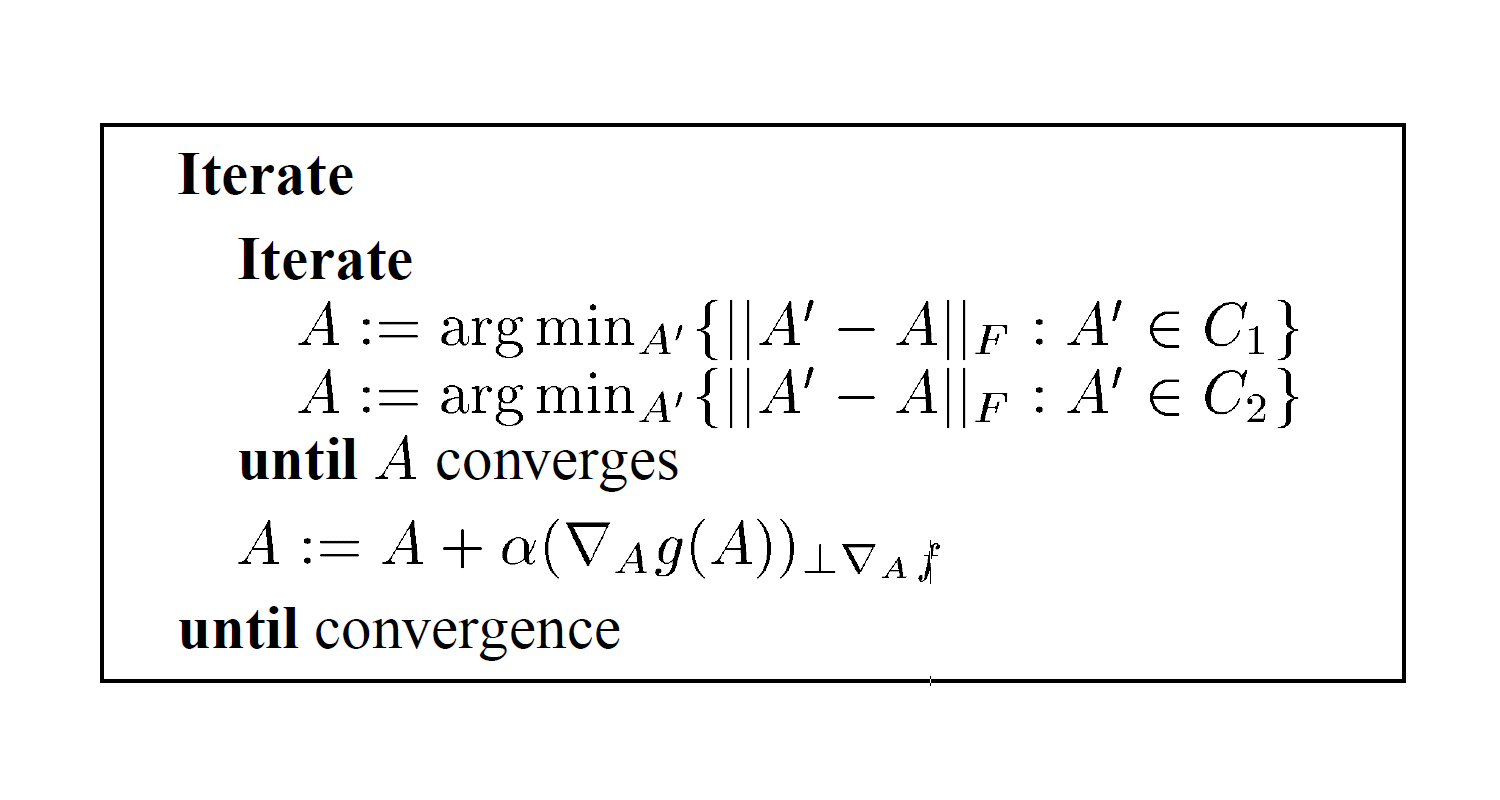
\includegraphics[width=0.6\linewidth]{Xing_algo}
\end{figure}
\vspace{-5mm}
where $C_1$ is the constraint
\[\sum_{(i,j) \in \M} \|x_i - x_j\|_A^2 \leq 1.\]
and $C_2$ is the constraint $A \succeq 0$.
}

\subsection{Experimental Results}
\subsection{Examples of learned metrics}
\frame{\frametitle{Examples of learned metrics}
Learning $A$ can be thought of as finding a linear transformation of the data
$x \mapsto \sqrt{A} x$ that moves similar pairs together:
\vspace{-2mm}
\begin{figure}[h!]
\centering
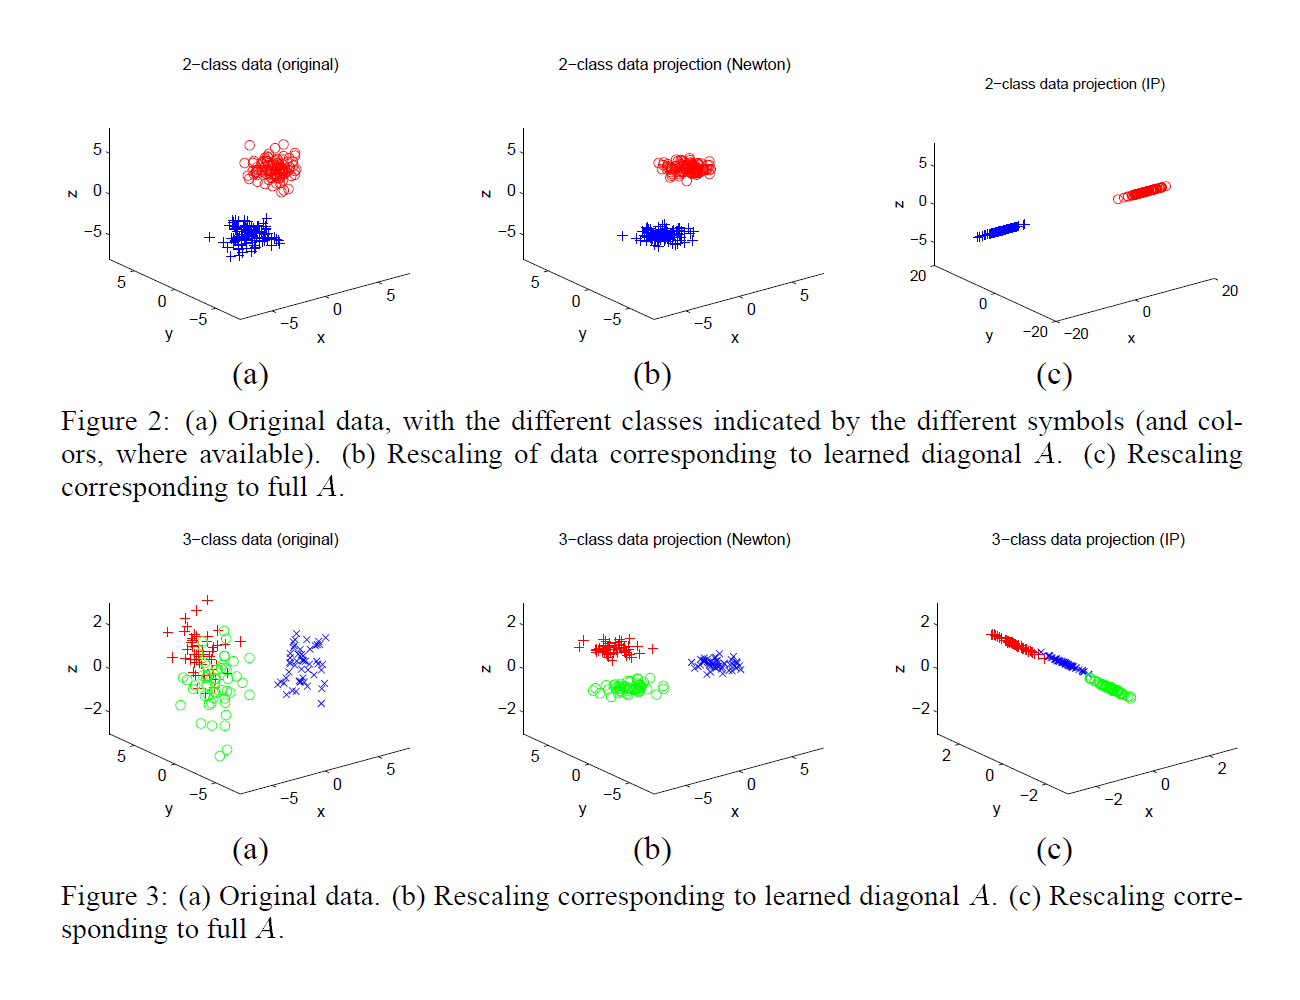
\includegraphics[width=0.75\linewidth]{lin_trans}
\end{figure}
\vspace{-5mm}
}

\subsection{Test Results}
\frame{\frametitle{Algorithms Tested}
\vspace{-2mm}
\hspace{-50mm}
\begin{figure}[h!]
\centering
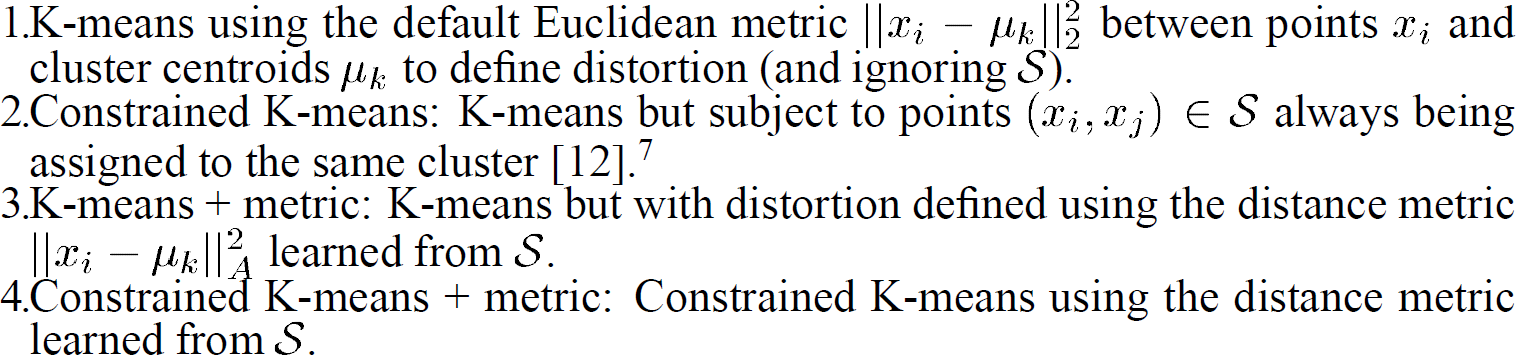
\includegraphics[width=1\linewidth]{all_algos}
\end{figure}
\vspace{-5mm}
}

\frame{\frametitle{Test Results}
\vspace{-2mm}
\hspace{-50mm}
\begin{figure}[h!]
\centering
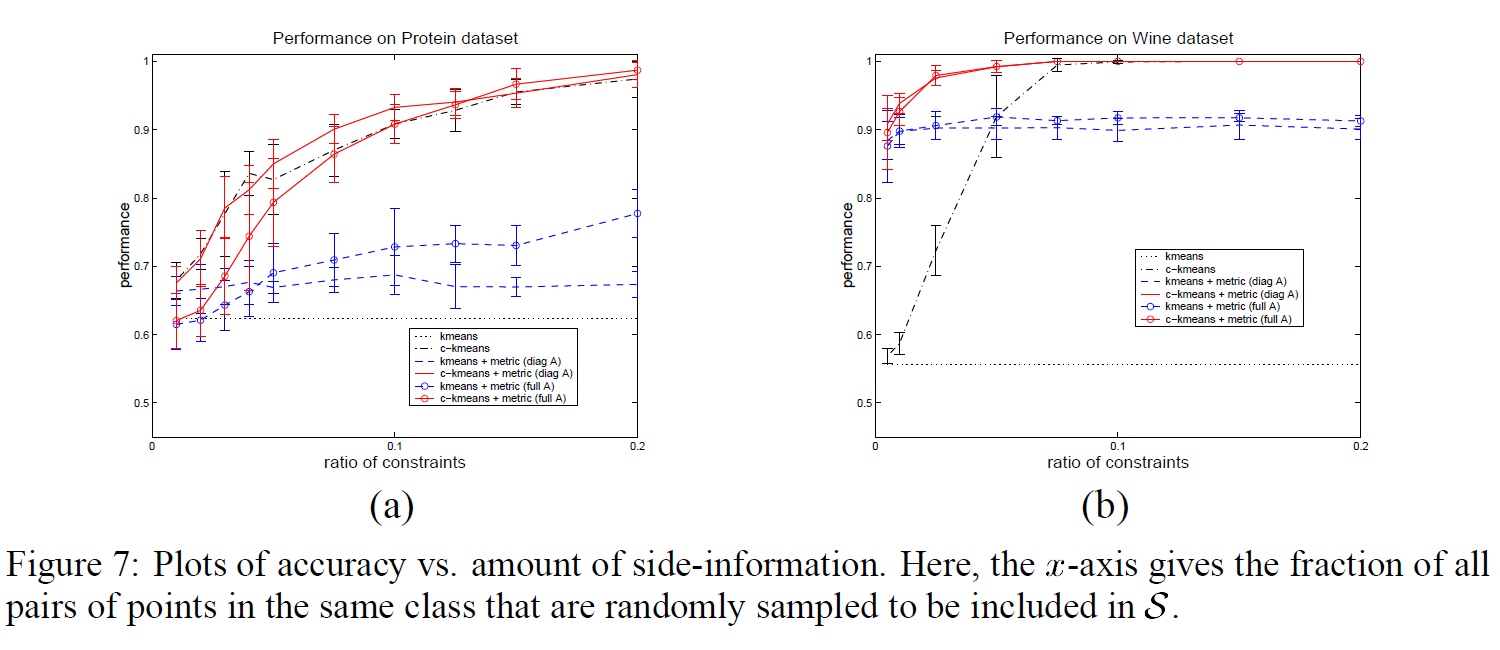
\includegraphics[width=1.1\linewidth]{protein_and_wine}
\end{figure}
\vspace{-5mm}
}

\section{Bilenko, et al.}
\subsection{Iterative Procedure}
\frame{\frametitle{Approach}
Previous metric-based semi-supervised clustering algorithms\ldots
\begin{itemize}
\item 
use only labeled data for metric learning step and separate metric learning
from clustering step
\item
learn a single metric for the entire data set
\item force satisfaction of all constraints
\end{itemize}

Algorithms takes an iterative (EM) approach, alternating between
\begin{enumerate}[1.]
\item clustering the entire dataset according to constraints and current
metric(s)
\item updating metric(s) according to current constraint violations
\end{enumerate}
}

\subsection{Pairwise Constraints}
\frame{\frametitle{Pairwise Constrainted $K$-Means (PCK-means)}
Minimize the $K$-means objective plus costs of constraint violations:
\[\sum_{i = 1}^n \|x_i - \mu_{\ell_i}\|_2^2
    + \sum_{(i,j) \in \M} w_{ij} 1_{\{\ell_i \neq \ell_j\}}
    + \sum_{(i,j) \in \C} w_{ij} 1_{\{\ell_i = \ell_j\}}
\]
}

\subsection{Multiple Metrics}
\frame{\frametitle{Multiple Metric $K$-Means (MK-means)}
Learning separate metrics for each cluster better adapts to varied cluster
shapes.

\vspace{5mm}
For each metric $\|x - y\|_{A_{\ell_i}} = \sqrt{(x - y)^TA_{\ell_i}(x - y)}$,
minimize
\[\sum_{i = 1}^n \|x_i - \mu_{\ell_i}\|_2^2
    - \log(\det(A_{\ell_i}))\]
(subject to $A \succeq 0$)
}

\subsection{Integrating Constraints and Metric Learning}
\frame{\frametitle{Integrating Constraints and Metric Learning}
Combining the previous objectives gives
\begin{align*}
\min_{A_1,\ldots,A_K \succeq 0,\ell} \quad\quad
 &  \sum_{i = 1}^n \|x_i - \mu_{\ell_i}\|_{A_{\ell_i}}^2 - \log(\det(A_{\ell_i}))  \\
    + & \sum_{(i,j) \in \M} w_{ij} 1_{\{\ell_i \neq \ell_j\}}
    + \sum_{(i,j) \in \C} w_{ij} 1_{\{\ell_i = \ell_j\}}
\end{align*}
\pause
This weights constraints independently of the distance between the
corresponding points.
}

\frame{\frametitle{Distance weighting}
To learn a good metric $d$
\begin{itemize}
\item 
violations of $(i,j) \in \M$ constraints should cost more when $d(x_i,x_j)$ is
large
\item 
violations of $(i,j) \in \C$ constraints should cost more when $d(x_i,x_j)$ is
small
\end{itemize}
Define
\[f_M(x_i,x_j)
    = \frac12\|x_i - x_j\|_{A_{\ell_i}}^2 + \frac12\|x_i - x_j\|_{A_{\ell_j}}^2
\]
and
\[f_M(x_i,x_j)
    = \|x_{\ell_i}' - x_{\ell_i}''\|_{A_{\ell_i}}^2 - \|x_i - x_j\|_{A_{\ell_i}}^2
\]
where
\[(x_{\ell_i}',x_{\ell_i}'')
    = \arg\!\!\!\!\max_{(x,y) \in \X} \|x - y\|_{A_{\ell_i}}.
\]
}

\frame{\frametitle{Integrating Constraints and Metric Learning}
Combining the previous objectives gives
\begin{align*}
\min_{A_1,\ldots,A_K \succeq 0,\ell} \quad\quad
 &  \sum_{i = 1}^n \|x_i - \mu_{\ell_i}\|_{A_{\ell_i}}^2 - \log(\det(A_{\ell_i}))  \\
    + & \sum_{(i,j) \in \M} w_{ij} f_M(x_i,x_j) 1_{\{\ell_i \neq \ell_j\}}
    + \sum_{(i,j) \in \C} w_{ij} f_C(x_i,x_j) 1_{\{\ell_i = \ell_j\}}
\end{align*}
}

\subsection{EM Procedure}
\frame{\frametitle{E-step}
\begin{itemize}
\item Sequentially add points greedily to cluster minimizing objective
\item Theoretically depends on ordering
\item Empirically, order does not matter much, so use random ordering
\end{itemize}
}

\frame{\frametitle{M-step}
\begin{itemize}
\item 
Can set gradient of objective w.r.t. $A_h$ to $0$ and solve for $A$ to get
closed form update
\item Project onto positive semidefinite cone (eliminates EM convergence
guarantee, but works empirically)
\item Requires inverting a $d \times d$ matrix, so can be too slow ($O(d^6)$)
in high dimensions
\item Restricting $A_h$ to be diagonal is more efficient (will see performance
later)
\end{itemize}
}

\frame{\frametitle{Initialization}
\begin{itemize}
\item 
Good initialization is critical for greedy algorithms such as $K$-means.
\item
Use constraints to infer initial constraints as follows:
\begin{enumerate}[1.]
\item Augment $\M$ with its transitive closure to create $\lambda$ cliques
\item Augment $\C$ with full bipartite graph between cliques with at least one
edge
\item If $\lambda < K$, add $K - \lambda$ random centroids
\item If $\lambda > K$, run farthest-first algorithm weighted by clique
size
\end{enumerate}
\end{itemize}
}

\subsection{Experimental Results}
\frame{\frametitle{Algorithms Tested}
\vspace{-8mm}
\begin{figure}[h!]
\centering
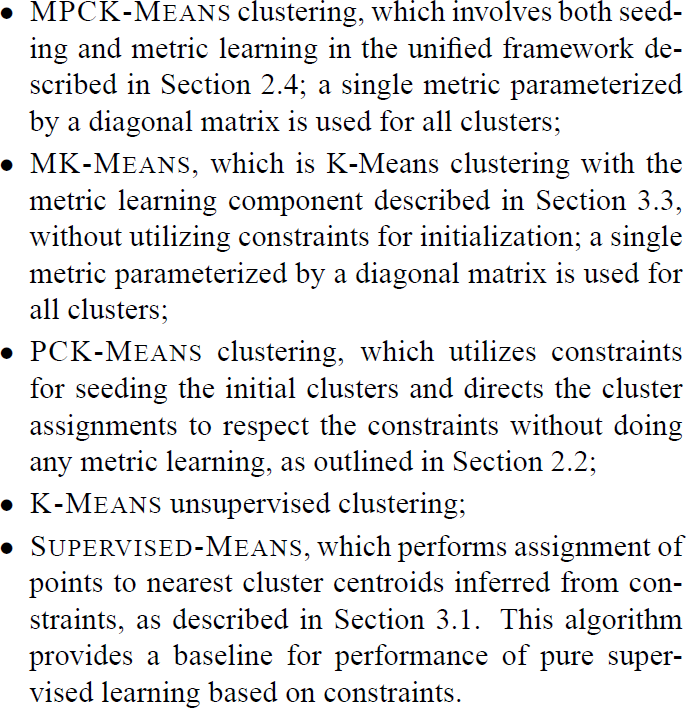
\includegraphics[width=0.4\linewidth]{all_algos2}
\end{figure}
}

\frame{\frametitle{Empirical Observations}
\begin{itemize}
\item Randomly sampled true labels to get constraints
\item Performance measured via $F$-measure (combination of precision and recall)
\item Generally, MPCK-means performed best
\end{itemize}
}

\frame{\frametitle{Empirical Observations}
Tried variants with single metric or diagonal $A$'s
\begin{itemize}
\item Fitting full matrix and multiple metrics generally performed best for
many constraints ($\approx 300$)
\item For smaller number of constraints, performance varied by data set
\end{itemize}
}

\section{Questions}
\frame{\frametitle{Questions}
Both two papers learn a metric from data and cluster. Xing does the two tasks
separately and Bilenko does them simultaneously. Xing does not use unlabeled
data to learn the metric and Bilenko uses unlabeled data via a clustering
framework which is based on k-means. Is there any other work that does metric
learning solely (like Xing) but also utilizes unlabeled data (i.e., a true
semi-supervised metric learning framework)?
\pause
\vspace{5mm}
Need to make an assumption about how unlabeled data should affect the metric.
Bilenko assumes the metric should conform to the clusters.
}

\end{document}
